\documentclass[12pt,letterpaper]{article}
\usepackage[utf8]{inputenc}
\usepackage[spanish]{babel}
\usepackage{graphicx}
\usepackage[left=2cm,right=2cm,top=2cm,bottom=2cm]{geometry}
\usepackage{graphicx} % figuras
% \usepackage{subfigure} % subfiguras
\usepackage{float} % para usar [H]
\usepackage{amsmath}
%\usepackage{txfonts}
\usepackage{stackrel} 
\usepackage{multirow}
\usepackage{enumerate} % enumerados
\renewcommand{\labelitemi}{$-$}
\renewcommand{\labelitemii}{$\cdot$}
% \author{}
% \title{Caratula}
\begin{document}

% Fancy Header and Footer
% \usepackage{fancyhdr}
% \pagestyle{fancy}
% \cfoot{}
% \rfoot{\thepage}
%

% \usepackage[hidelinks]{hyperref} % CREA HYPERVINCULOS EN INDICE

% \author{}
\title{Caratula}

\begin{titlepage}
\begin{center}
\large{UNIVERSIDAD PRIVADA DE TACNA}\\
\vspace*{-0.025in}
\begin{figure}[htb]
\begin{center}

\includegraphics[width=7cm]{./images/logo}
\end{center}
\end{figure}
\vspace*{0.15in}
INGENIERIA DE SISTEMAS  \\

\vspace*{0.3in}
\begin{large}
\textbf{TITULO:} \\
\end{large}

\vspace*{0.1in}
\begin{Large}
\textbf{INFORME DE LABORATORIO 05 -   Elaboración de consultas sobre un Cubo Multidimensional en SQL Server} \\
\end{Large}

\vspace*{0.3in}
\begin{Large}
\textbf{CURSO:} \\
\end{Large}

\vspace*{0.1in}
\begin{large}
INTELIGENCIA DE NEGOCIOS\\
\end{large}

\vspace*{0.3in}
\begin{Large}
\textbf{DOCENTE:} \\
\end{Large}

\vspace*{0.1in}
\begin{large}
 Ing. Patrick Cuadros Quiroga\\
\end{large}

\vspace*{0.4in}
\vspace*{0.1in}
\begin{large}
\textbf{Estudiante:} \\
\begin{flushleft}
Sharon Sosa Bedoya  \hfill	(2016054460)\\

\centering  %CENTRA UN TEXTO
\vspace*{0.9in}
\begin{large}
Tacna\\ 
\end{large}

\end{flushleft}
\end{large}
\end{center}

\end{titlepage}


\tableofcontents % INDICE
\thispagestyle{empty} % INDICE SIN NUMERO
\newpage
\setcounter{page}{1} % REINICIAR CONTADOR DE PAGINAS DESPUES DEL INDICE



\section{Ejercicio 1 - Creacion de un proyecto de Analisys Services}  

Antes de comenzar este ejercicio debera crear:

Una carpeta en el escritorio con el nombre: Proyecto2CuboCarnet

1. Crear un nuevo Proyecto en Visual Studio 2019 , Hacer clic en Business Intelligence.

	\begin{center}
	
\includegraphics[width=\columnwidth]{images/task1/img1}
	\end{center}	


2. Seleccione el tipo de Proyecto multidimensional y de minería de datos de Analysis Services
	\begin{center}
	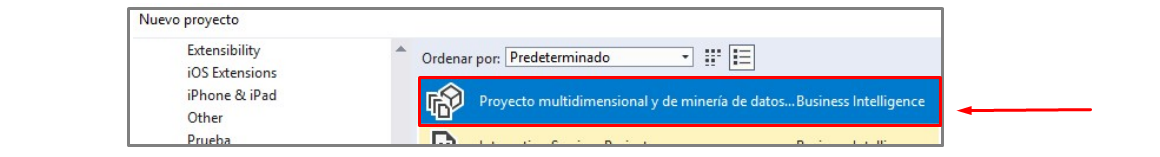
\includegraphics[width=\columnwidth]{images/task1/img2}
	\end{center}	

3. Colocar como nombre de proyecto: CuboAdventureWorks2012
		
4. Seleccionar la carpeta creada en el escritorio

	\begin{center}
	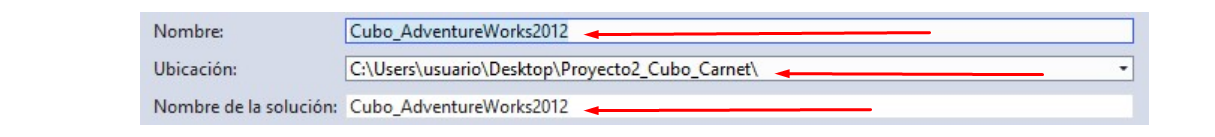
\includegraphics[width=\columnwidth]{images/task1/img4}
    \end{center}	

5. . Hacer clic en Aceptar

    
\section{Ejercicio 2 - Creación del cubo}  



1. Utilice la base de datos AdventureWorksDW2012 como origen de datos

	\begin{center}
	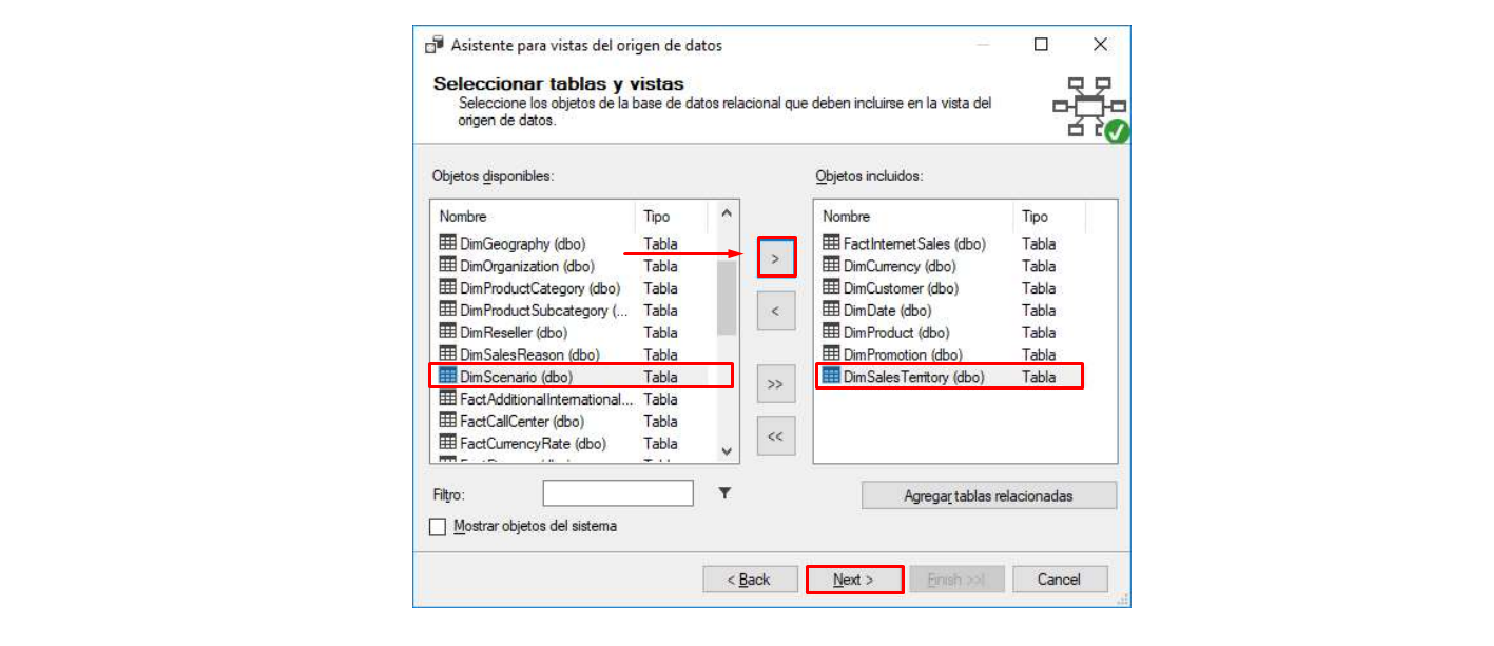
\includegraphics[width=\columnwidth]{images/task2/img1}
	\end{center}	


2. En la opción definir una vista del origen de datos seleccione las siguientes tablas de la base de datos:
FactInternetSales, DimCurrency, DimCustomer, DimDate, DimProduct, DimPromotion, DimSalesTerritory

	\begin{center}
	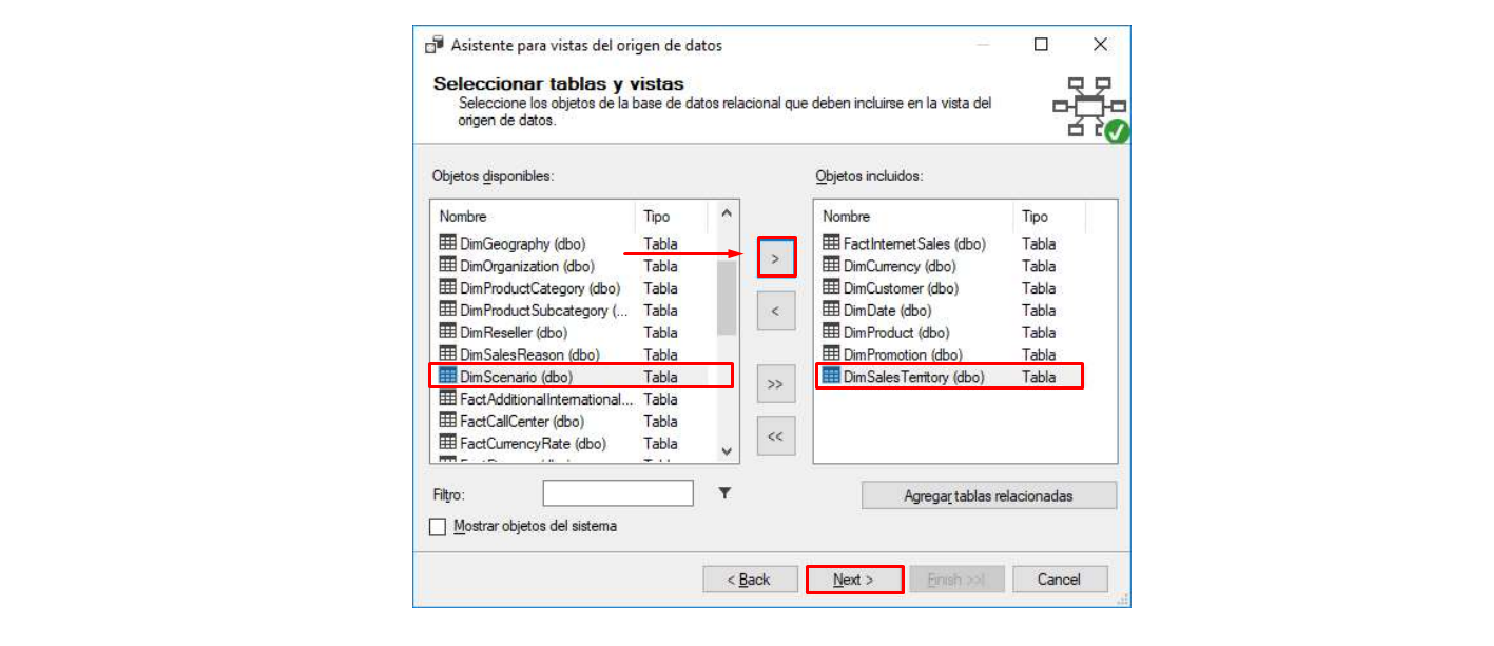
\includegraphics[width=\columnwidth]{images/task2/img2}
	\end{center}	

	\begin{center}
	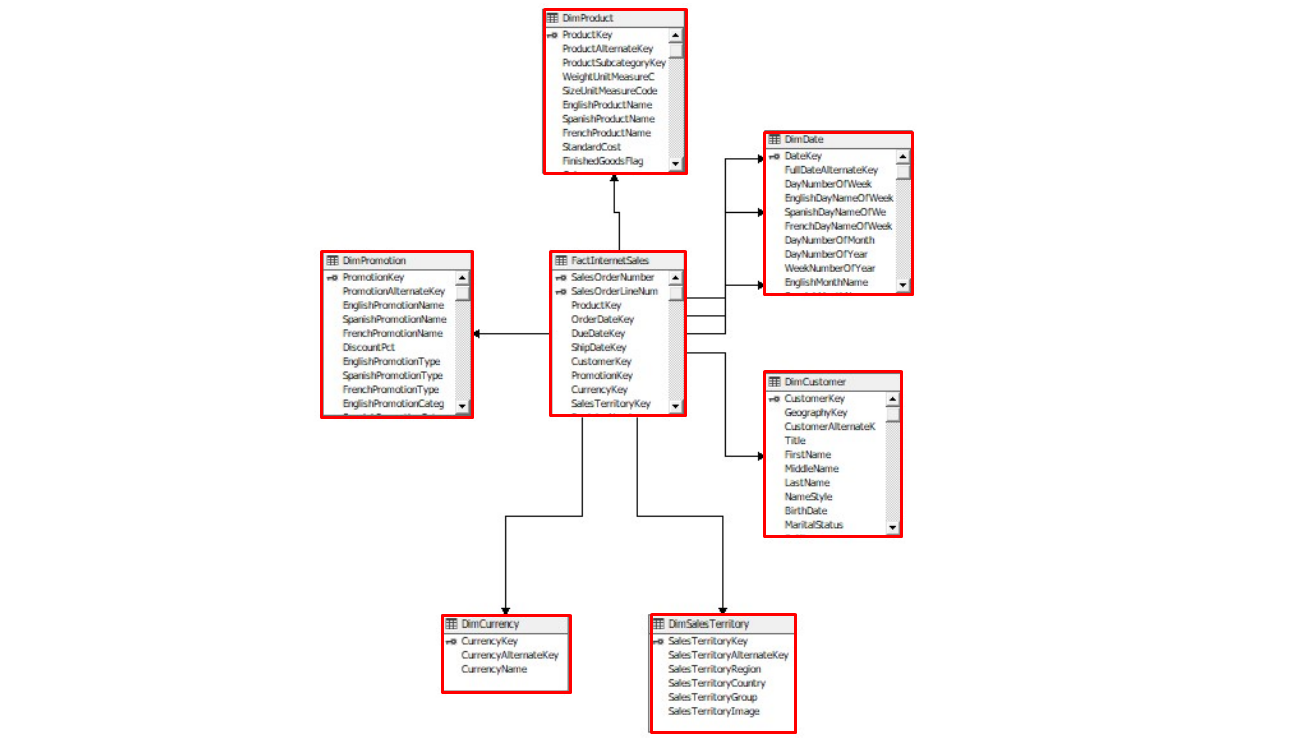
\includegraphics[width=\columnwidth]{images/task2/img3}
	\end{center}	

3. Crear un cubo tomando en cuenta las tablas del origen de datos

	\begin{center}
	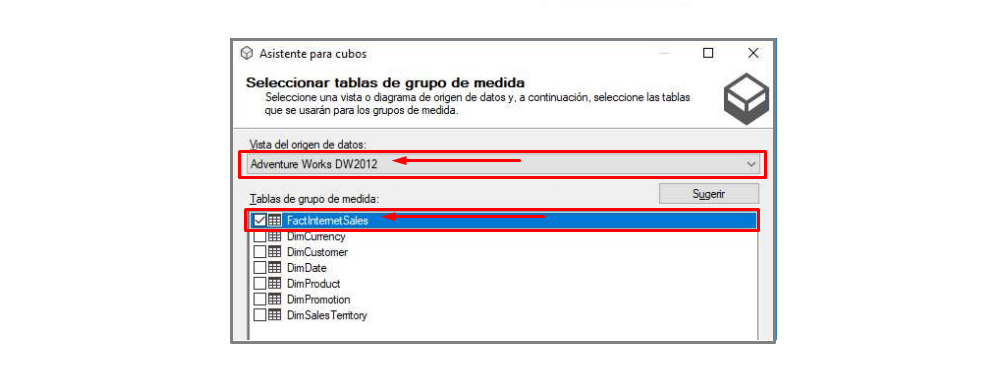
\includegraphics[width=\columnwidth]{images/task2/img4}
    \end{center}	

	\begin{center}
	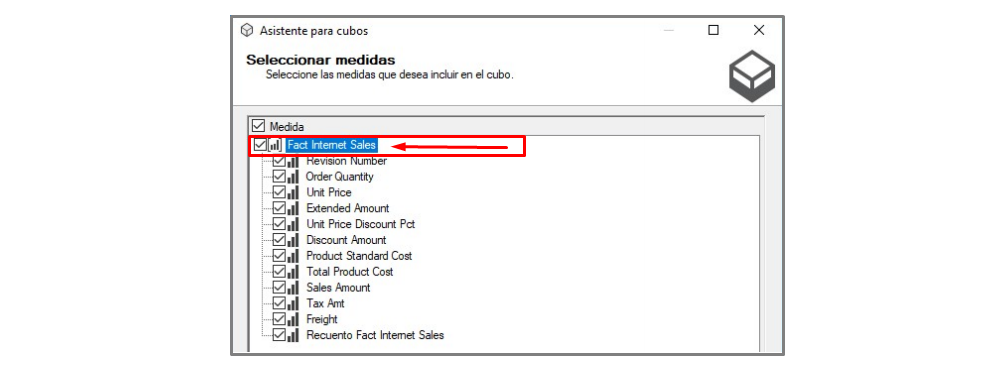
\includegraphics[width=\columnwidth]{images/task2/img5}
    \end{center}	
		
	Procesar el cubo y Examinar el cubo.

4. Cambiar la dimensión Date a:

	\begin{center}
	
\includegraphics[width=\columnwidth]{images/task2/img6}
    \end{center}	



    
\section{Ejercicio 3 - Configurar el Name Column en una Dimensión}  

1. En las propiedades del atributo Product Key nos ubicamos en NameColumn:

	\begin{center}
	
\includegraphics[width=\columnwidth]{images/task1/img1}
	\end{center}	


2. Nos abrirá una ventana donde podemos enmascarar este atributo por otro, en este caso seleccionaremos el
atributo EnglishProductName:

	\begin{center}
	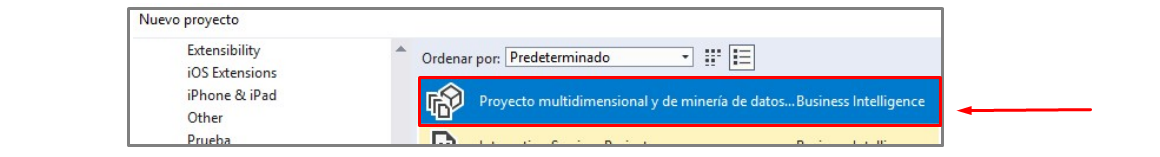
\includegraphics[width=\columnwidth]{images/task1/img2}
	\end{center}	

Click en Ok.

3. Eliminaremos el atributo EnglishProductName y renombraremos el atributo Product Key por Product:

	\begin{center}
	
\includegraphics[width=\columnwidth]{images/task1/img3}
	\end{center}	

Procesamos la dimensión DimProduct.

4. Una vez procesada la dimensión nos volvemos a Reconcetar al mismo:

	\begin{center}
	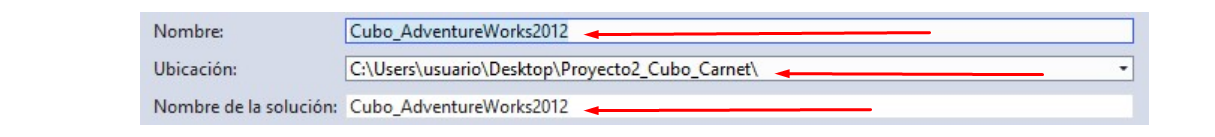
\includegraphics[width=\columnwidth]{images/task1/img4}
    \end{center}	

5. Si ahora consultamos el atributo Product obtendremos lo siguiente:

	\begin{center}
	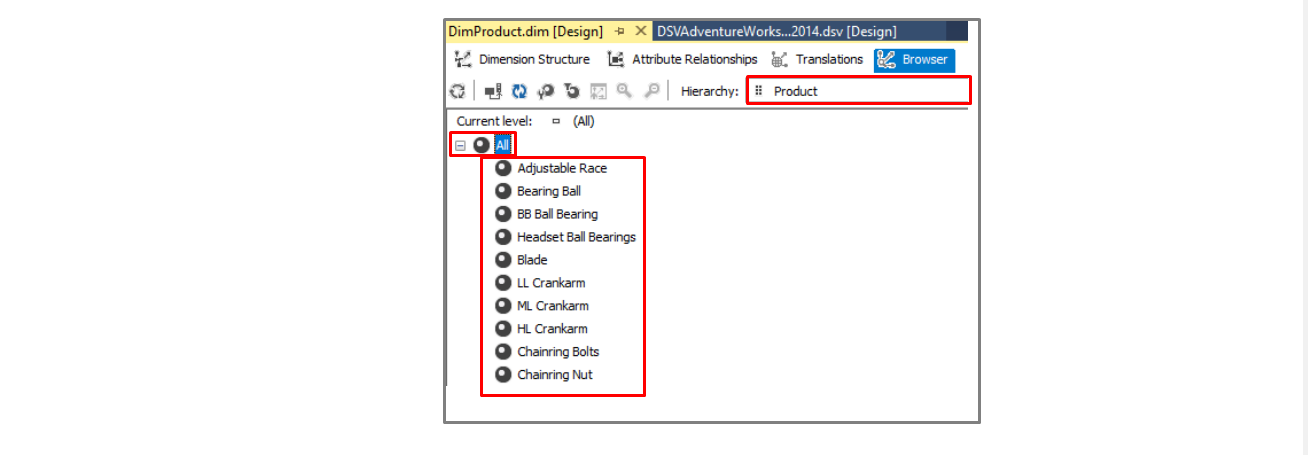
\includegraphics[width=\columnwidth]{images/task1/img5}
    \end{center}	


    
\section{Ejercicio 4 - Usar el cálculo con nombre para los nombres de miembro}  

1. Haga doble clic en la dimensión DimDate en el nodo Dimensiones del Explorador de soluciones.

2. En el panel Atributos de la pestaña Estructura de dimensión, haga clic en el atributo Date Key

	\begin{center}
	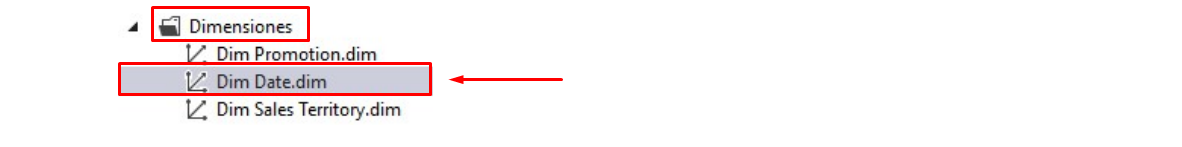
\includegraphics[width=\columnwidth]{images/task4/img1}
	\end{center}	

3.Haga clic en el campo de la propiedad NameColumn y, a continuación, haga clic en el botón de puntos suspensivos
(…) para abrir el cuadro de diálogo Columna de nombre.
	\begin{center}
	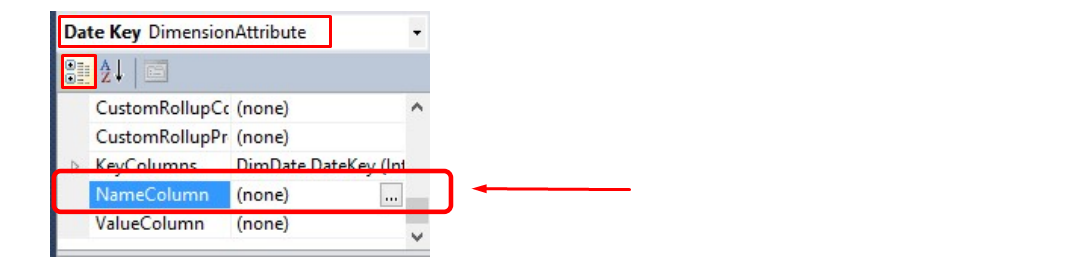
\includegraphics[width=\columnwidth]{images/task4/img2}
	\end{center}	

4. Seleccione SimpleDate en la lista Columna de origen y, a continuación, haga clic en Aceptar.

	\begin{center}
	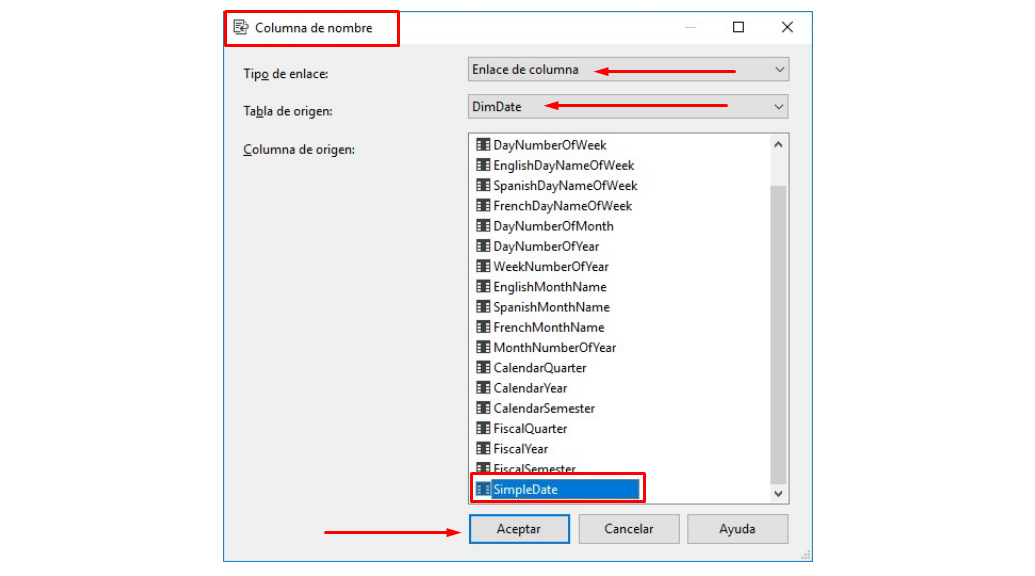
\includegraphics[width=\columnwidth]{images/task4/img3}
	\end{center}	

5. En el menú Archivo del proyecto, haga clic en Guardar todo

    
\section{Ejercicio 5 - Crear una jerarquía}  

1. En el Diseñador de dimensiones para la dimensión DimDate, arrastre el atributo Calendar Year del panel
Atributos al panel Jerarquías

	\begin{center}
	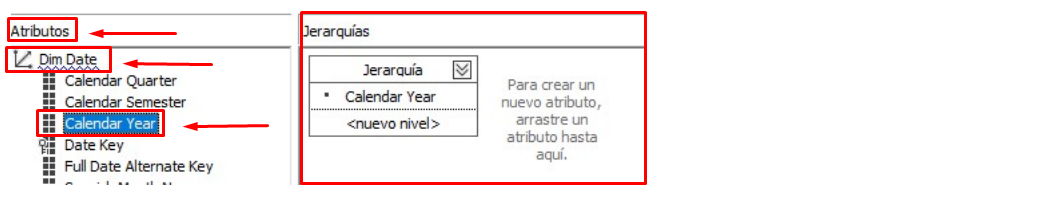
\includegraphics[width=\columnwidth]{images/task5/img1}
	\end{center}	

2. Arrastre el atributo Calendar Semester del panel Atributos a la celda <nuevo nivel> del panel Jerarquías, debajo
del nivel Calendar Year

3.Arrastre el atributo Calendar Quarter del panel Atributos a la celda <nuevo nivel> del panel Jerarquías, debajo
del nivel Calendar Semester.

4. Arrastre el atributo Spanish Month Name del panel Atributos a la celda <nuevo nivel> del panel Jerarquías, debajo del nivel Calendar Quarter.

5. Arrastre el atributo Date Key del panel Atributos a la celda <nuevo nivel> del panel Jerarquías, debajo del nivel
Spanish Month Name.

	\begin{center}
	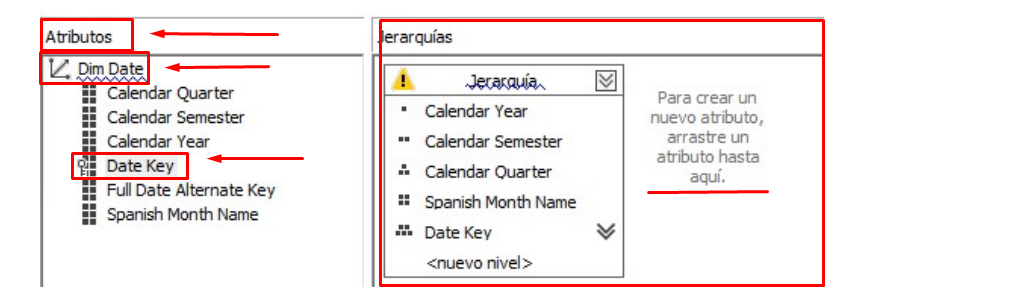
\includegraphics[width=\columnwidth]{images/task5/img2}
	\end{center}	

6. En el panel Jerarquías, haga clic derecho en la barra de título de la jerarquía Jerarquía, seleccione Cambiar nombre
y escriba Calendar Date.

7. En la jerarquía Calendar Date, cambie el nombre del nivel Spanish Month Name a Calendar Month y el del nivel
Date Key a Date.

	\begin{center}
	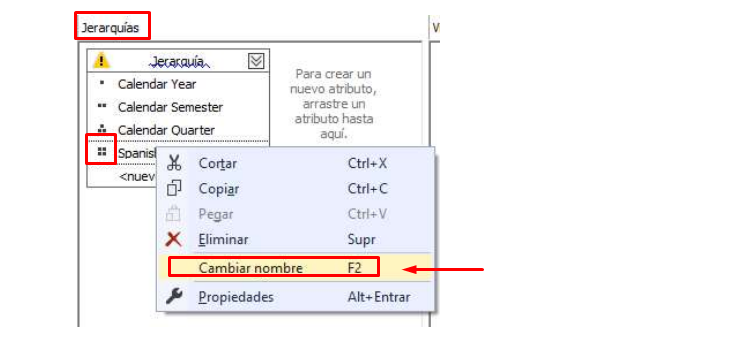
\includegraphics[width=\columnwidth]{images/task5/img3}
	\end{center}	

	\begin{center}
	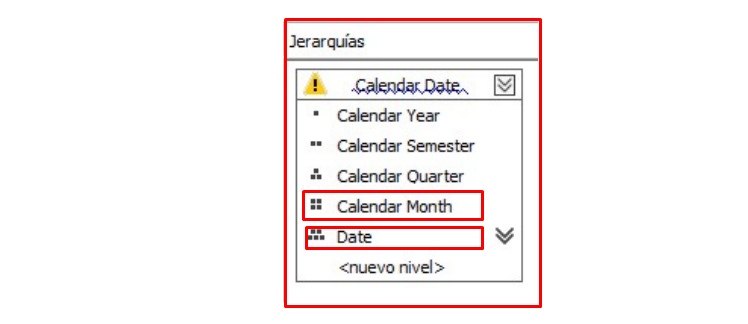
\includegraphics[width=\columnwidth]{images/task5/img4}
	\end{center}	

8. Elimine el atributo FullDateAlternateKey del panel Atributos, ya que no lo va a usar.

	\begin{center}
	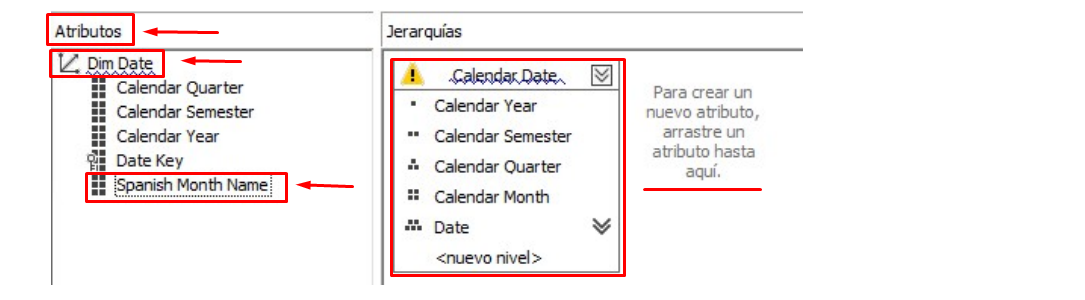
\includegraphics[width=\columnwidth]{images/task5/img5}
	\end{center}	

9. Verificar las relaciones del atributo DateKey en la pestaña Realaciones de atributo

	\begin{center}
	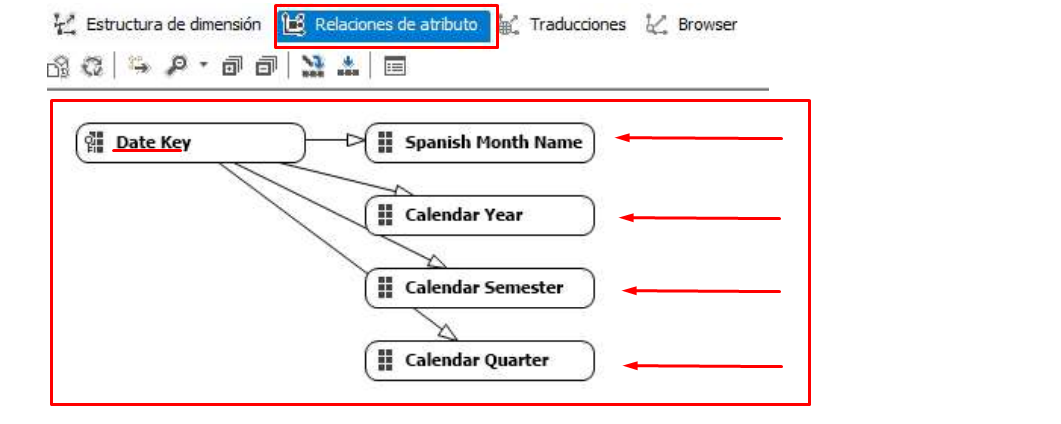
\includegraphics[width=\columnwidth]{images/task5/img6}
	\end{center}	

10. En el menú Archivo del proyecto, haga clic en Guardar todo

    
\section{Ejercicio 6 - Proporcionar nombres de miembros de dimensión únicos}  

1. Haga clic en la carpeta Vistas del origen de datos en el Explorador de soluciones, después haga doble clic en el
origen de datos Adventure Works DW2012.dsv

2. En el panel Tablas, haga clic derecho en DimDate y, a continuación, haga clic en Nuevo cálculo con nombre

3. En el cuadro de diálogo Crear cálculo con nombre, escriba MonthName en el cuadro Nombre de columna y, a
continuación, escriba la siguiente instrucción en el cuadro Expresión:

	\begin{center}
	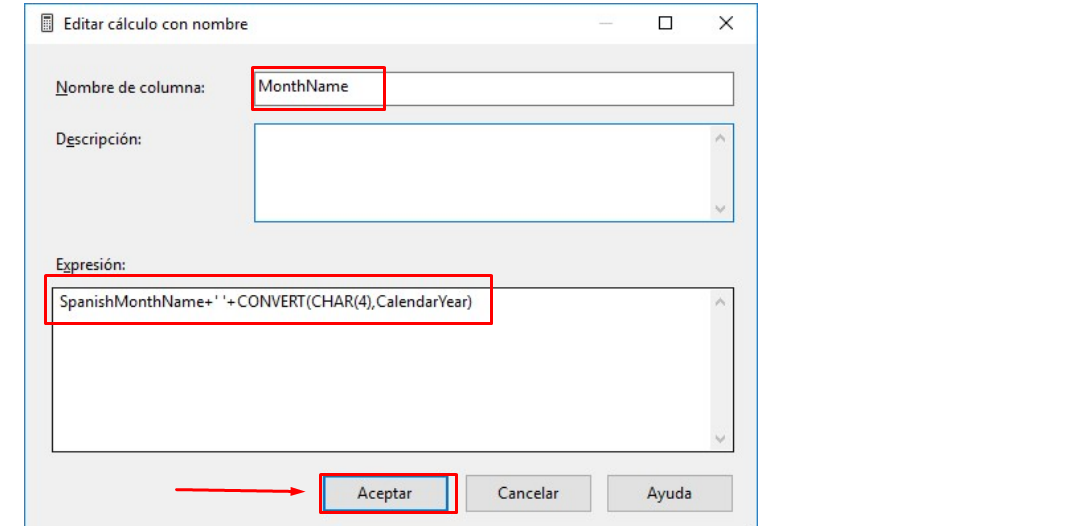
\includegraphics[width=\columnwidth]{images/task6/img1}
	\end{center}	

4. Esta instrucción concatena el mes y el año de cada mes de la tabla a una nueva columna.

5. Haga clic en Aceptar

6. En el panel Tablas, haga clic derecho DimDate y, a continuación, haga clic en Nuevo cálculo con nombre

7. En el cuadro de diálogo Crear cálculo con nombre, escriba CalendarQuarterDesc en el cuadro Nombre de
columna y, a continuación, escriba el script SQL siguiente en el cuadro Expresión:

	\begin{center}
	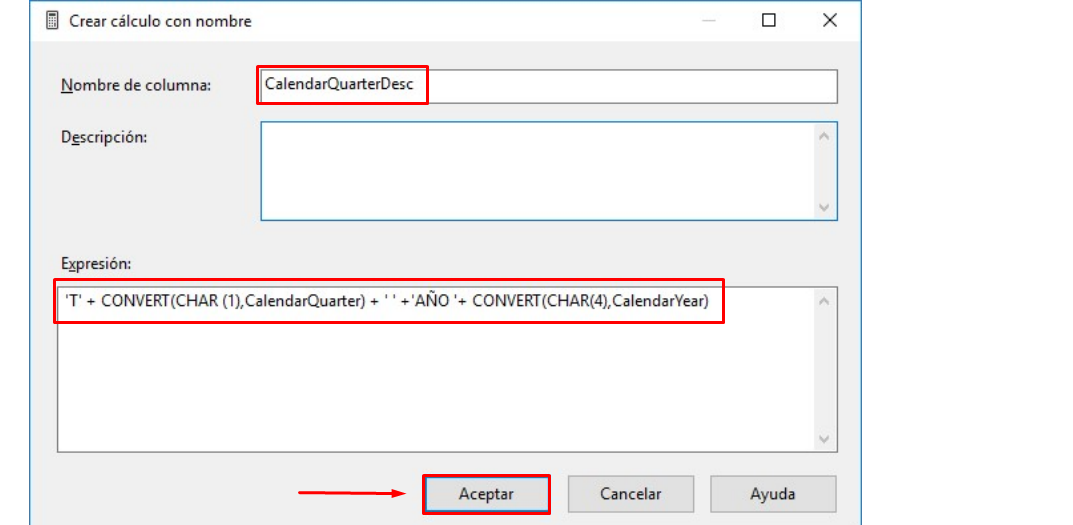
\includegraphics[width=\columnwidth]{images/task6/img2}
	\end{center}	

8. Este script SQL concatena el trimestre natural y el año de cada trimestre de la tabla en una nueva columna.

9. Haga clic en Aceptar

10. Haga clic derecho sobre la dimensión DimDate y seleccione la opción Explorar datos y al final de la tabla puede
observar la siguiente información:

	\begin{center}
	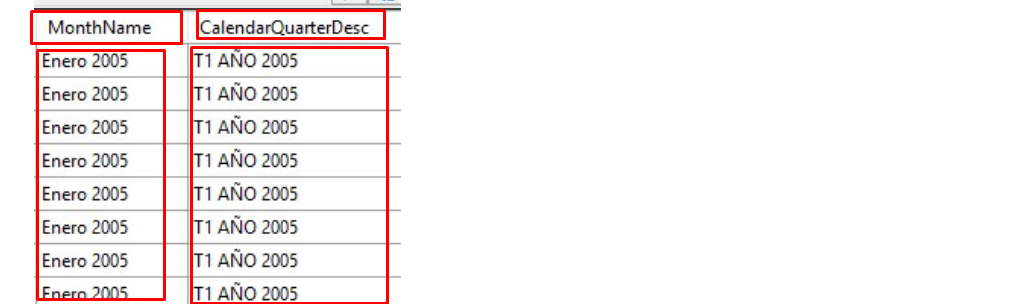
\includegraphics[width=\columnwidth]{images/task6/img3}
	\end{center}	

11. En el panel Tablas, haga clic derecho en DimDate y, a continuación, haga clic en Nuevo cálculo con nombre

12. En el cuadro de diálogo Crear cálculo con nombre, escriba CalendarSemesterDesc en el cuadro Nombre de
columna y, a continuación, escriba el script SQL siguiente en el cuadro Expresión:

	\begin{center}
	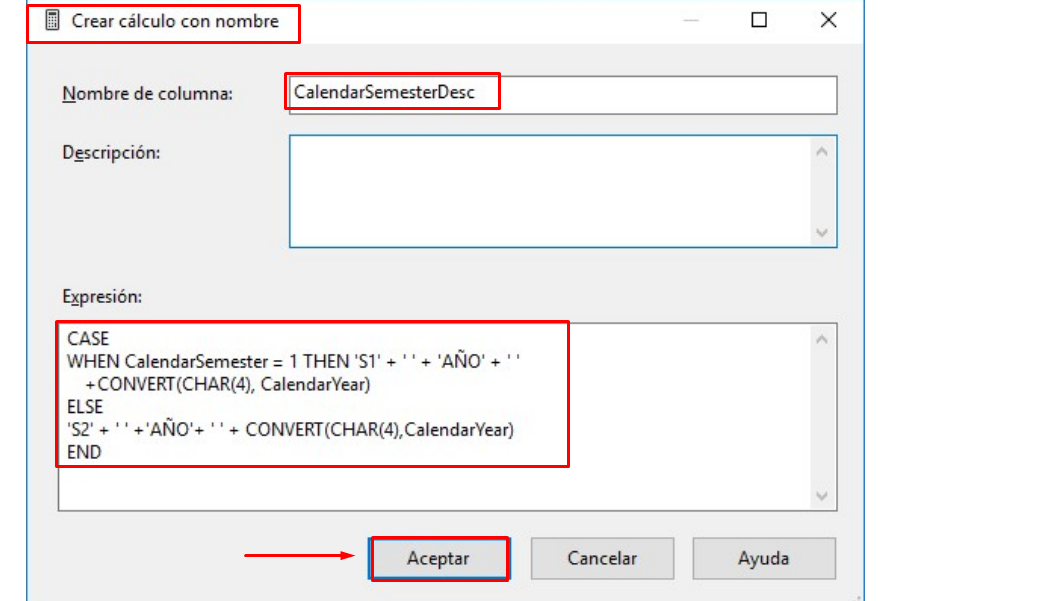
\includegraphics[width=\columnwidth]{images/task6/img4}
	\end{center}	

13. Este script SQL concatena el semestre natural y el año de cada semestre de la tabla en una nueva columna.

14. Haga clic en Aceptar

15. En el menú Archivo del proyecto, haga clic en Guardar todo

16. Haga clic derecho sobre la dimensión DimDate y seleccione la opción Explorar datos y al final de la tabla puede
observar la siguiente información:

	\begin{center}
	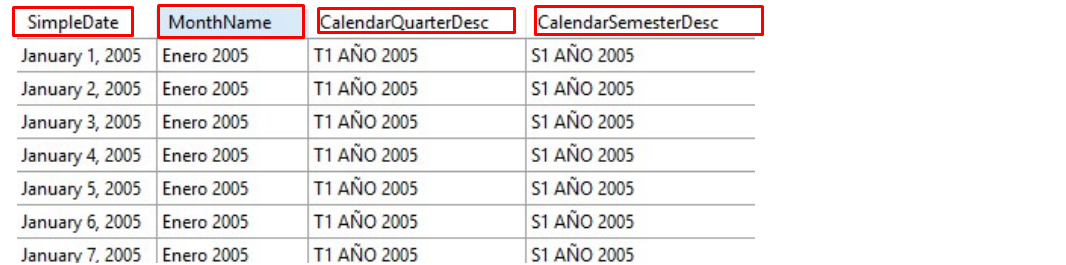
\includegraphics[width=\columnwidth]{images/task6/img5}
	\end{center}	

17. Cerrar todas las pestañas

18. Procesar el cubo, hacer clic en la opción SI, indicando que el cubo ha cambiado desde su última implementación

19. Examinar el cubo

	\begin{center}
	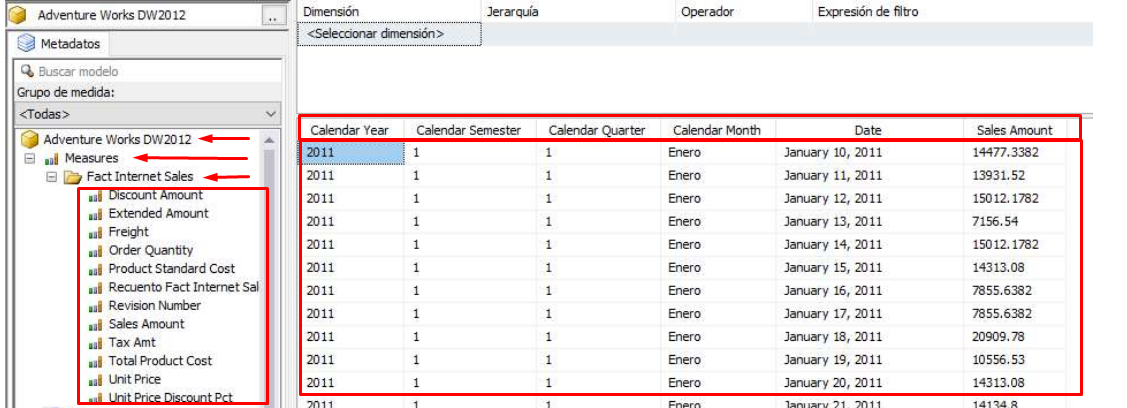
\includegraphics[width=\columnwidth]{images/task6/img6}
	\end{center}	
\section{Ejercicio 7 - Definir cálculos}  

1. Abra el Diseñador de cubos y, a continuación, haga clic en la pestaña Cálculos
Observe el comando predeterminado CALCULATE en el panel de las expresiones de cálculo y en el panel
Organizador de scripts. Este comando especifica que las medidas del cubo deberían agregarse según el valor
especificado por sus propiedades AggregateFunction. Los valores de medida normalmente se suman, pero
también pueden contarse o agregarse de otra forma.

	\begin{center}
	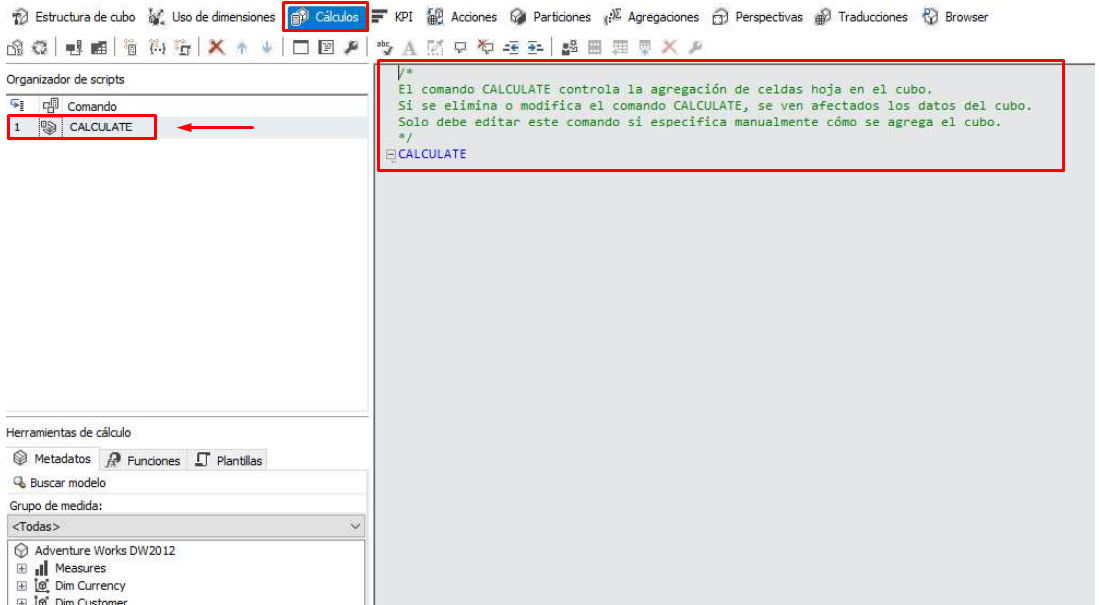
\includegraphics[width=\columnwidth]{images/task7/img1}
	\end{center}	

2. En la barra de herramientas de la pestaña Cálculos, haga clic en Nuevo miembro calculado
En el panel de las expresiones de cálculo aparece un nuevo formulario en el que podrá definir las propiedades de
este nuevo miembro calculado. El nuevo miembro aparecerá también en el panel Organizador de scripts. La siguiente imagen muestra el formulario que aparece en el panel de las expresiones de cálculo al hacer clic en Nuevo miembro calculado

	\begin{center}
	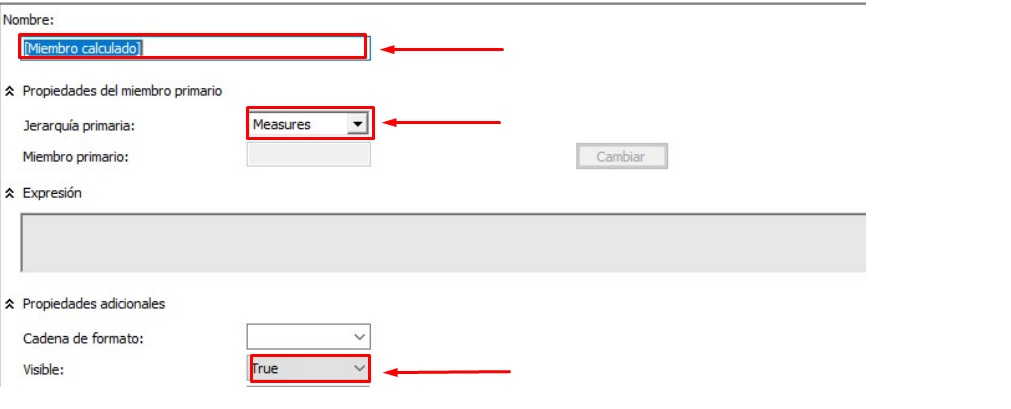
\includegraphics[width=\columnwidth]{images/task7/img2}
	\end{center}	

3. En el cuadro Nombre, cambie el nombre de la medida calculada por [Total de Ventas].
Si el nombre de un miembro calculado contiene un espacio, dicho nombre deberá ir entre corchetes.
Observe que en la lista Jerarquía primaria, de manera predeterminada, se crea un nuevo miembro calculado en
la dimensión Measures. A un miembro calculado de la dimensión Measures también se le denomina con
frecuencia medida calculada.

4. En la pestaña Metadatos del panel Herramientas de cálculo

	\begin{center}
	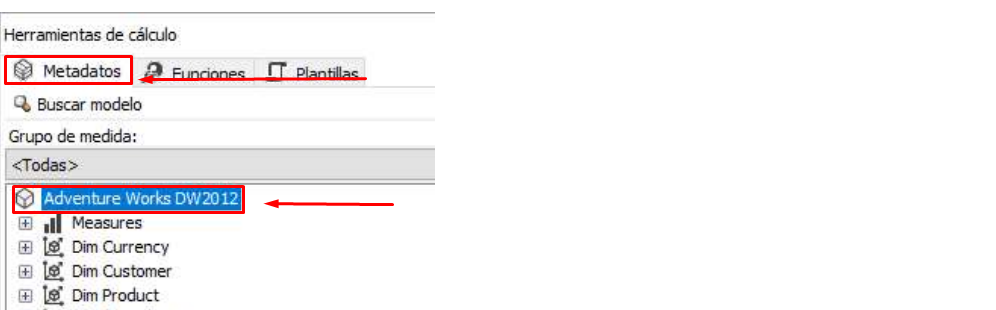
\includegraphics[width=\columnwidth]{images/task7/img3}
	\end{center}	

5.Expanda Medidas (Measures) y, a continuación, FactInternet Sales para ver los metadatos del grupo de medida
FactInternet Sales.

	\begin{center}
	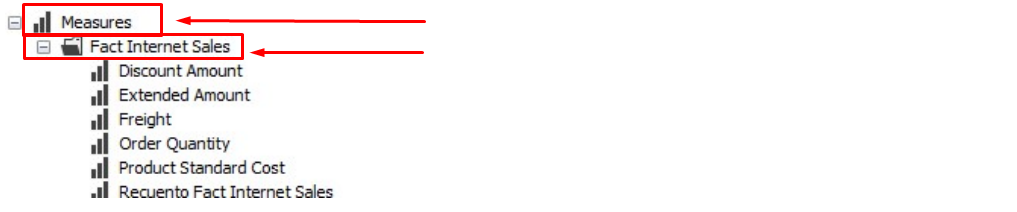
\includegraphics[width=\columnwidth]{images/task7/img4}
	\end{center}	

Puede arrastrar los elementos de metadatos desde el panel Herramientas de cálculo al cuadro Expresión y
agregar entonces operadores y otros elementos para crear expresiones multidimensionales (MDX). O bien, puede
escribir la expresión MDX directamente en el cuadro Expresión

	\begin{center}
	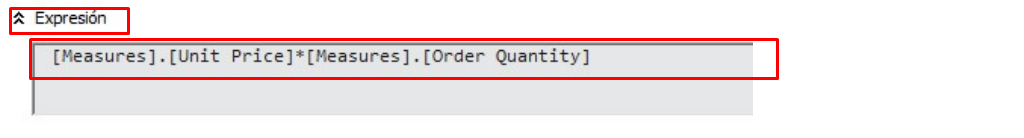
\includegraphics[width=\columnwidth]{images/task7/img5}
	\end{center}	

6. En la lista Cadena de formato, seleccione "Currency"

7. En la lista Comportamiento si no está vacío, active las casillas de verificación Unit Price y haga clic en Aceptar.

	\begin{center}
	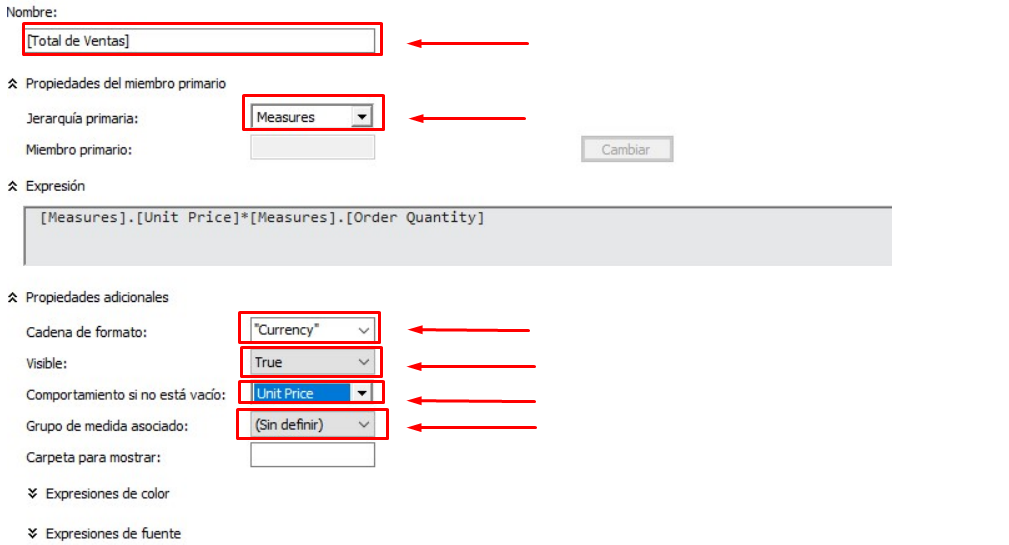
\includegraphics[width=\columnwidth]{images/task7/img6}
	\end{center}	

Las medidas especificadas en la lista Comportamiento si no está vacío se utilizan para resolver consultas NON
EMPTY en MDX. Si se especifican una o más medidas en la lista Comportamiento si no está vacío, Analysis Services
tratará al miembro calculado como vacío si todas las medidas especificadas están vacías. Si la propiedad Nonempty behavior está en blanco, Analysis Services deberá evaluar al miembro calculado para determinar si el
miembro está vacío.

8. En la barra de herramientas de la pestaña Cálculos, haga clic en Vista de script y revise la script del cálculo
en el panel de las expresiones de cálculo.

	\begin{center}
	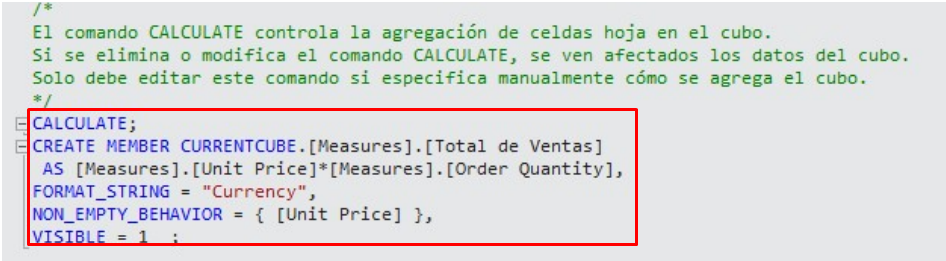
\includegraphics[width=\columnwidth]{images/task7/img7}
	\end{center}	

Observe que el nuevo cálculo se agrega a la expresión CALCULATE inicial; los cálculos individuales se separan con
un punto y coma. Observe también que aparece un comentario al principio de la script del cálculo. Se recomienda
la agregación de comentarios dentro de la script de cálculo para grupos de cálculos para ayudarle a usted y a otros
programadores a comprender las scripts de cálculo complejas.

9. Guardar los cambios

10. Cerrar el diseñador del cubo

11. Procesar el cubo

12. Examinar el cubo

13. Abrir el diseñador del Cubo y en la pestaña Cálculos en la opción de Grupo de medida observe el nuevo miembro
calculado

	\begin{center}
	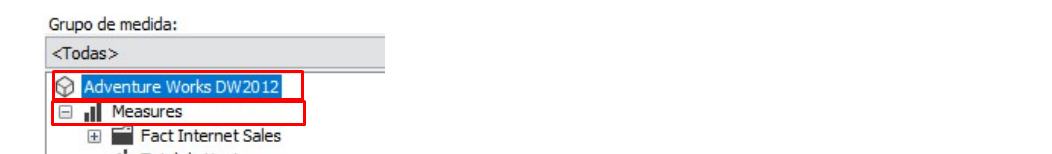
\includegraphics[width=\columnwidth]{images/task7/img8}
	\end{center}	

\subsection{Definir cálculos de margen de beneficio bruto}  

1. Haga clic en Nuevo miembro calculado en la barra de herramientas de la pestaña Cálculos. 

2. En el cuadro Nombre, cambie el nombre de esta nueva medida calculada por [Porcentaje Costo Producto].

3. En el cuadro Expresión, cree la siguiente expresión MDX:

[Measures].[Total Product Cost]/[Measures].[Sales Amount]

4. Verifique las propiedades adicionales, así como se muestra en la siguiente imagen

	\begin{center}
	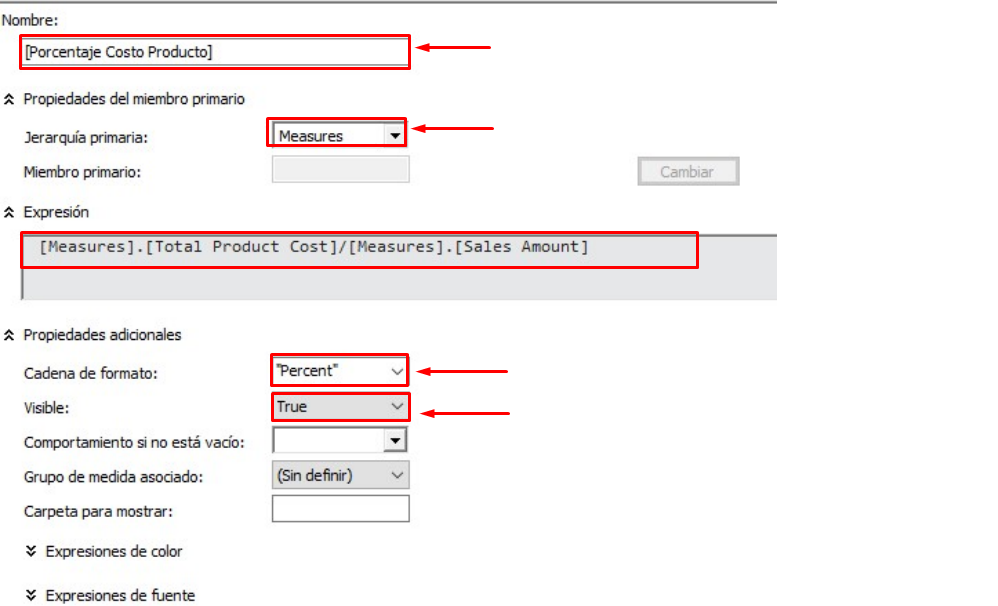
\includegraphics[width=\columnwidth]{images/task7/img9}
	\end{center}	


5. Guardar los cambios al proyecto

6. Cerrar el diseñador del cubo

7. Procesar el cubo

8. Examinar el cubo

9. Abrir el diseñador del Cubo y en la pestaña Cálculos en la opción de Grupo de medida observe el nuevo miembro
calculado

	\begin{center}
	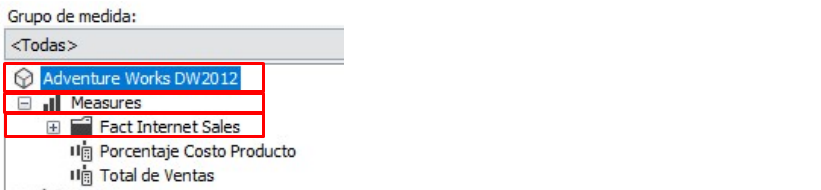
\includegraphics[width=\columnwidth]{images/task7/img10}
	\end{center}	


La siguiente imagen muestra el panel Script View con los cálculos creados.

	\begin{center}
	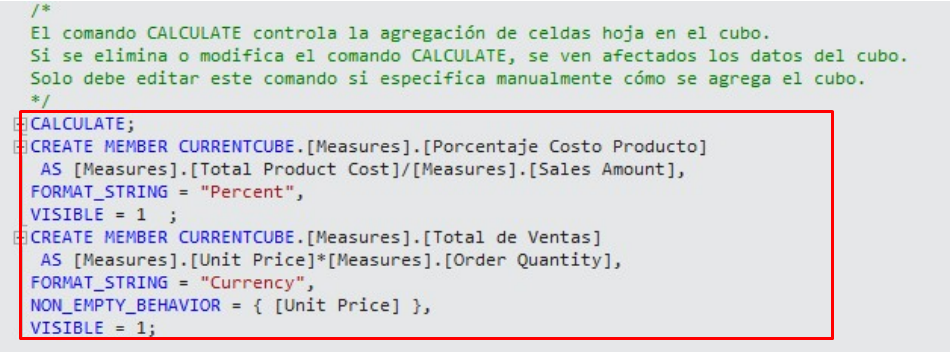
\includegraphics[width=\columnwidth]{images/task7/img11}
	\end{center}	


\subsection{Examinar los nuevos miembros calculados}  

1. Hacer clic en la pestaña Browser

2. Arrastrar los nuevos campos calculados para verificar su funcionamiento, así como se muestra a continuación:

	\begin{center}
	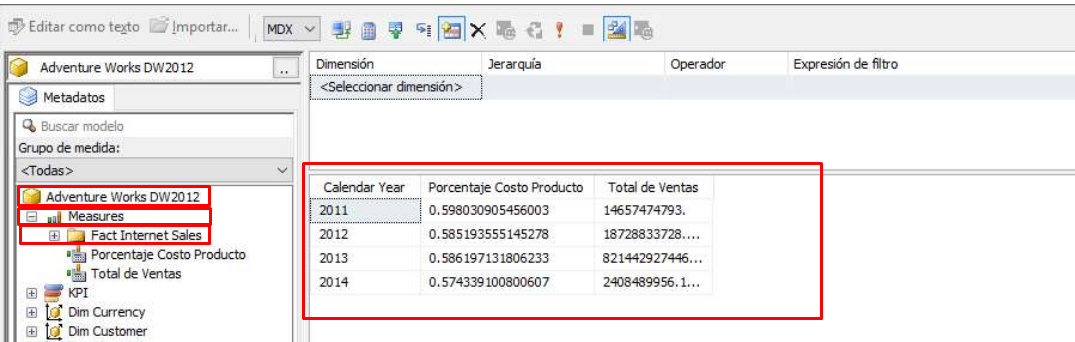
\includegraphics[width=\columnwidth]{images/task7/img12}
	\end{center}	

\section{Ejercicio 8 - Definir indicadores clave de rendimiento (KPI)}  

1.Cambiarse a la pestaña KPI La pestaña KPI incluye varios paneles. En la parte izquierda de la pestaña están el panel Organizador de KPI y el panel Herramientas de cálculo. El panel de muestra del centro de la pestaña contiene los detalles del KPI seleccionado en el panel Organizador de KPI. La siguiente imagen muestra la pestaña KPI del Diseñador de cubos

	\begin{center}
	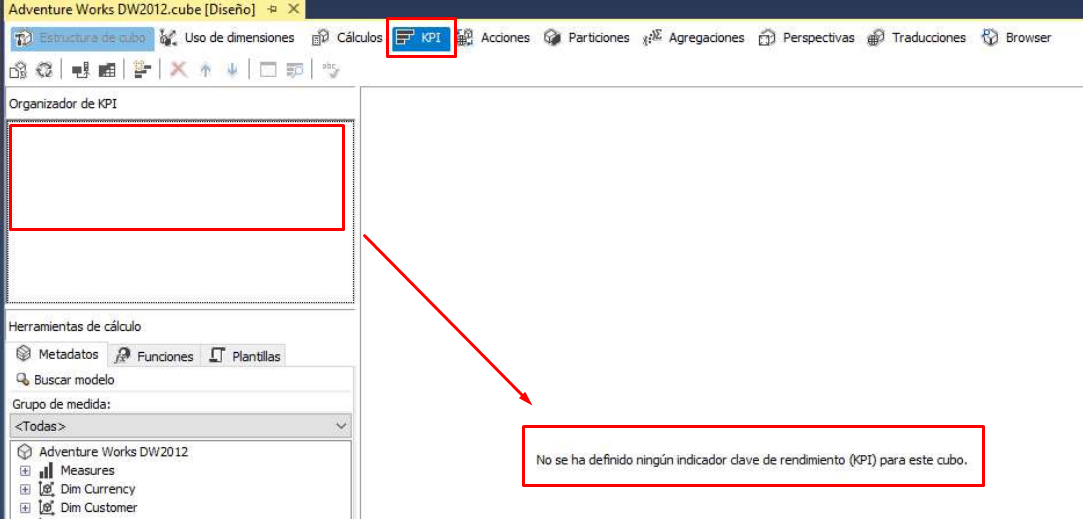
\includegraphics[width=\columnwidth]{images/task8/img1}
	\end{center}	

2. En la barra de herramientas de la pestaña KPI, haga clic en el botón Nuevo KPI en el panel de muestra aparecerá una plantilla de KPI en blanco, como en la siguiente imagen.

	\begin{center}
	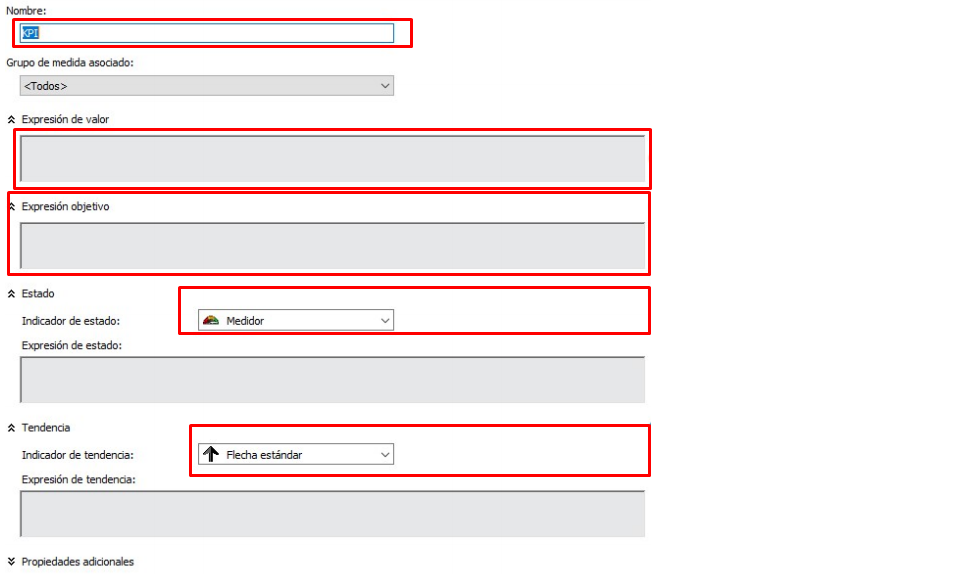
\includegraphics[width=\columnwidth]{images/task8/img2}
	\end{center}	

3. En el cuadro Nombre, escriba Venta y, a continuación, seleccione Fact Internet Sales en la lista Grupo de medida
asociado

4. En la pestaña Metadatos del panel Herramientas de cálculo, expanda Medidas

	\begin{center}
	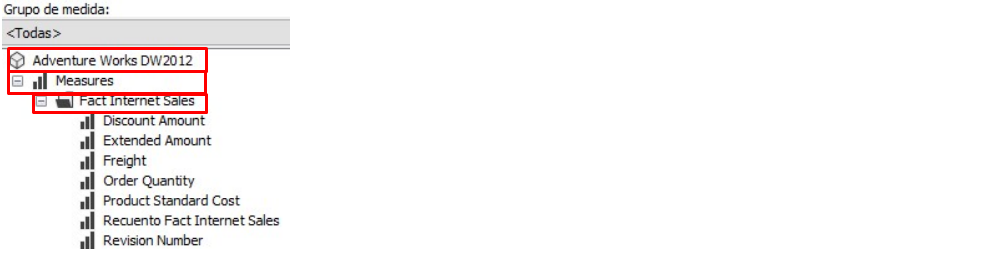
\includegraphics[width=\columnwidth]{images/task8/img3}
	\end{center}	


5. Expanda la tabla Fact Internet Sales y, a continuación, arrastre la medida Sales Amount al cuadro Expresión de
valor.

	\begin{center}
	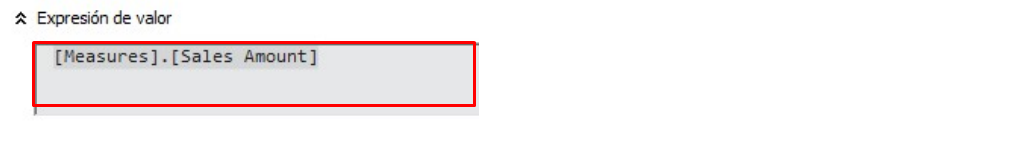
\includegraphics[width=\columnwidth]{images/task8/img4}
	\end{center}	


6. En el cuadro Expresión objetivo digite:

	\begin{center}
	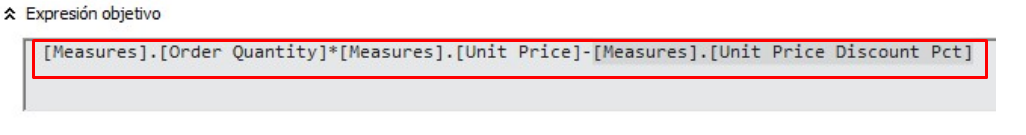
\includegraphics[width=\columnwidth]{images/task8/img5}
	\end{center}	

7. Compruebe que está seleccionado Indicador en la lista Indicador de estado, seleccione uno tal como se muestra
en la figura:

	\begin{center}
	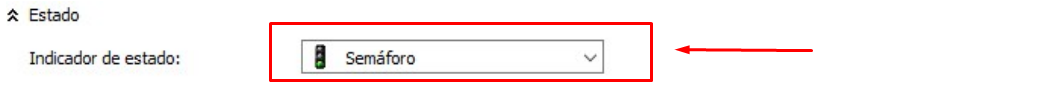
\includegraphics[width=\columnwidth]{images/task8/img6}
	\end{center}	

y, a continuación, escriba la siguiente expresión MDX en el cuadro Expresión de estado:

	\begin{center}
	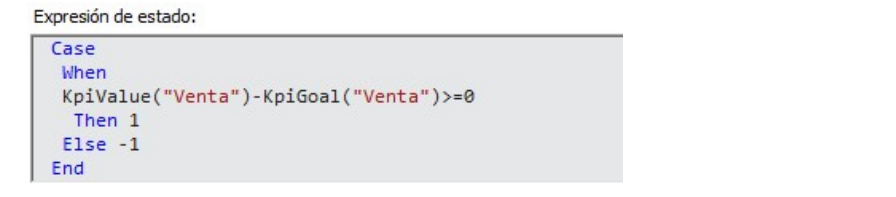
\includegraphics[width=\columnwidth]{images/task8/img7}
	\end{center}	


8. Compruebe que está seleccionado Flecha estándar en la lista Indicador de tendencia

	\begin{center}
	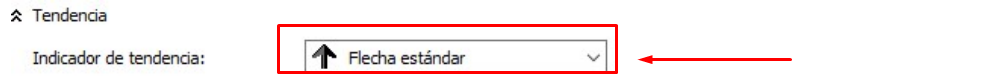
\includegraphics[width=\columnwidth]{images/task8/img8}
	\end{center}	

9. Y a continuación, escriba la siguiente expresión en el cuadro Expresión de tendencia:

	\begin{center}
	\includegraphics[width=\columnwidth]{images/task8/img9}
	\end{center}	


10. Guardar los cambios

11. Cerrar el diseñador del cubo

12. Procesar el cubo

\subsection{Examinar el cubo mediante el KPI}

1. Abrir el diseñador del cubo

2. Hacer clic en la pestaña KPI

	\begin{center}
	\includegraphics[width=\columnwidth]{images/task8/img10}
	\end{center}	

3. Luego haga clic en la opción Vista examinador.

4. En el panel Filtro, seleccione Order Date en la lista Dimensión

5. Seleccione Calendar Date en la lista Jerarquía, seleccione Igual en la lista Operador

	\begin{center}
	\includegraphics[width=\columnwidth]{images/task8/img11}
	\end{center}	

6. En la lista Expresión de filtro seleccione tal como se muestra a continuación:

	\begin{center}
	\includegraphics[width=\columnwidth]{images/task8/img12}
	\end{center}	

7. Y a continuación, haga clic en Aceptar

8. Arrastre el KPI al panel Examinador de KPI

	\begin{center}
	\includegraphics[width=\columnwidth]{images/task8/img13}
	\end{center}	

9. Para actualizar los valores para el KPI Venta, haga clic en el enlace “Haga clic para ejecutar la consulta”


	\begin{center}
	\includegraphics[width=\columnwidth]{images/task8/img14}
	\end{center}	


\end{document}